\subsection{Exploration}
Our results were limited to test run outside of gazebo. We were able to test the breath first search algorithm which provided an obtacle free path to a defined goal. The results of this test are shown in figure \ref{fig:a-star-map}. We also were able to test the robots motion model, the results of these tests revealed that the youbot was an ideal candidate since it was orientation agnostics and was fully holonomic. The one limitation to the youbot platform was its ability to traverse ramps, this was factored in when designing static characteristics as described in the methodology section. The motion model for the husky and the rosbot were far from ideal due to path deflection and turn radius.

\begin{figure}[H]
  \centering
    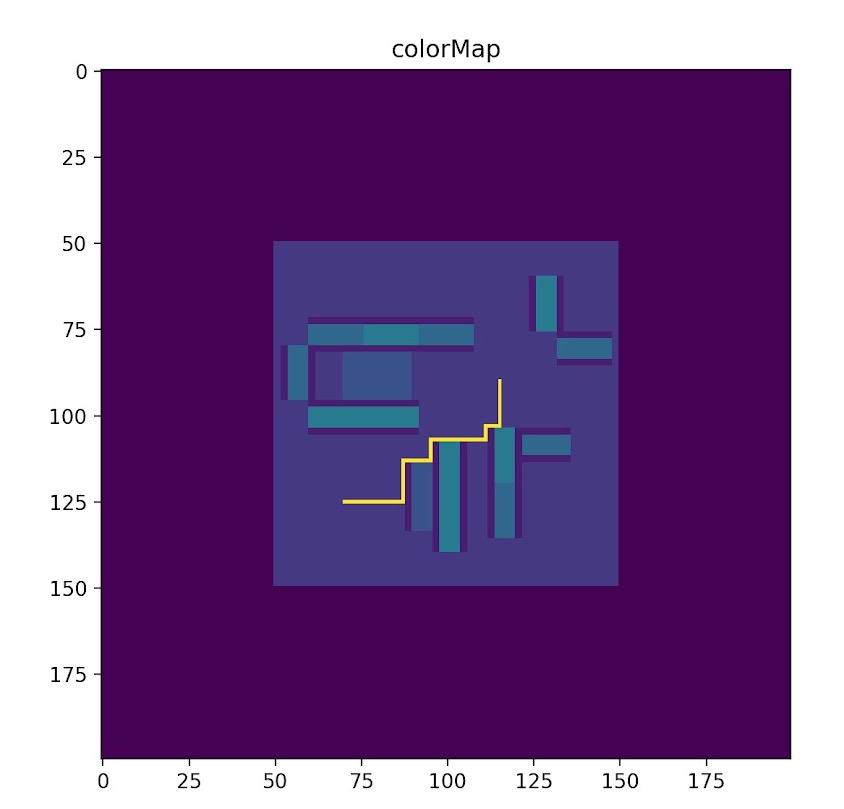
\includegraphics[width=0.5\textwidth]{a-star-map}
  \caption{A* python path planning simulation} \label{fig:a-star-map}
\end{figure}
